%% 美赛模板:正文部分

\documentclass[12pt]{article}  % 官方要求字号不小于 12 号,此处选择 12 号字体

% 本模板不需要填写年份,以当前电脑时间自动生成
% 请在以下的方括号中填写队伍控制号
\usepackage[2111259]{easymcm}  % 载入 EasyMCM 模板文件
\problem{D}  % 请在此处填写题号
%\usepackage{mathptmx}  % 这是 Times 字体,中规中矩
\usepackage[table,xcdraw]{xcolor}%更多色彩
\usepackage{tikz-network}%绘图宏包
\usetikzlibrary{shapes}%绘图宏包
\usepackage{mathpazo}  % 这是 COMAP 官方杂志采用的更好看的 Palatino 字体,可替代以上的 mathptmx 宏包
\usepackage{verbatim}%注释宏包

%\usepackage{tocloft} %模板中用了subfigure,不加此选项会产生冲突
%\renewcommand{\cftchapleader}{\cftdotfill{\cftdotsep}}
%\renewcommand{\cftsecleader}{\cftdotfill{\cftdotsep}}

\title{The study of the similarity of artists and their genres}  % 标题

% 如需要修改题头(默认为 MCM/ICM),请使用以下命令(此处修改为 MCM)
%\renewcommand{\contest}{MCM}

% 文档开始
\begin{document}

% 此处填写摘要内容
\begin{abstract}

Music evolves with social changes. To understand the role of music in the human collective experience,  the evolutionary and revolutionary trends of artists and genres following social changes are examined. 

For questions one and two, an \textbf{adjacency list} is constructed to describe the artist's music influence network. The relationship between influencers and followers is established \textbf{through the weighted method of directed paths}. Through the \textbf{recursive algorithm}, artist's "music influence" , that is, the \textby{"new generation talent influence"} is obtained. This parameter reveals the artist's attraction to new talents and contribution to the development of music. To determine the specific value of the path weight, we use the \textbf{modified cosine similarity algorithm} to obtain the similarity relationship between every two artists, and \textbf{use this as the weighting parameter of the graph}. On this basis, it is concluded that artists of the same type are more similar than artists of different types. 

For question three, the inter-genre and the inner-genre are analyzed separately. We found the average music characteristics of each genre and calculated the \textbf{similarity of the average characteristics of different genres} to get the difference of music characteristics between genres. At the same time, we calculate the \textbf{similarity of every two artists in the genre} to get the similarity ranking of the artists in the genre. Besides, we summed up the influence of music within the genre and found that the pop/rock genre has the greatest influence, and through the mapping of the music characteristics of each genre to the chronological analysis, we obtained the popular genre change table. 

For question four, we compare the average similarity between every two artists with the average similarity of direct influence and conclude the influence of those affected by fan creation. Furthermore, we calculated the \textbf{Pearson correlation coefficients} of various music characteristics, and found that the energy and acoustics music characteristics of the influencer were the most "infectious".

For questions five and six, similarity calculations are performed year by year, and music characteristics are analyzed for years with low similarity. Then, look for musicians with great musical influence in that year, and analyze the similarity between the musicians and the musical characteristics of that year. Take 1967 as an example, the Beatles has the most influence and has a high similarity with the musical characteristics of the changing year. Music revolutionaries. In addition, we use the \textbf{entropy method} to calculate the change weights of music characteristics in a ten-year interval. The larger the weight, the greater the degree of dispersion of the characteristics. Finally, we found that the energy and loudness characteristics of the pop/rock genre continued to rise after the 1960s, indicating that the pop/rock genre has become more active.

For question seven, we combined the cited relevant literature to analyze the mutual influence between music and culture. For music influence culture, the method of searching high-impact artists has been used. As for music embodies cultural changes, the data obtained in question six is the key to the Pop/Rock example.

    % 美赛论文中无需注明关键字。若您一定要使用,
    % 请将以下两行的注释号 '%' 去除,以使其生效
    \vspace{5pt}
    \textbf{Keywords}: cosine similarity, entropy, Pearson correlation coefficient

\end{abstract}

\maketitle  % 生成 Summary Sheet
\tableofcontents  % 生成目录

\newpage

% 正文开始
\section{Introduction}
\subsection{Problem Background}
Music is an art form whose medium is sound and silence.\cite{noauthor_music_nodate} In the thousand-year history of mankind, music is an indispensable part of the development of civilization. When artists are creating music, many factors affect them, including their musical creativity, personal experience, current hot news, and social status.\par
Sometimes, music also undergoes revolutionary changes, creating new sounds or rhythms, introducing a new genre and trend, or changing the pattern of existing genres. By analyzing song networks and their musical characteristics in different periods, we can begin to capture the influence of music artists on each other, understand the similarities and differences between and within genres, so as to better understand how music has evolved with social and cultural changes of. 
%\cite{1}引用
\subsection{Problem Restatement}
To examine artist genres and evolutionary trends, and build a model of musical influence. We have the following problems waiting to be solved:
\begin{itemize}
    \item Establish a music influence network to capture the parameters of "music impression". 
    \item Develop a music similarity measure. 
    \item Compare the relationship between artists within genres and between genres, and get the relationship between genres. 
    \item The role of music influencers on followers. 
    \item Find a revolution on the network that may mark the evolution of music. 
    \item Analyze the evolution of a genre over time and give an explanation. 
    \item Use models to express the cultural influence of music in time or environment, and identify the influence of socio-political or technological changes. 
\end{itemize}



%\begin{enumerate}[\bfseries 1.]
%    \item We do ...
%    \item We do ...
%    \item We do ...
%\end{enumerate}
%第二部分
\section{Basic Assumptions}
\begin{itemize}
    \item It is assumed that artists in the network can indirectly influence other artists through the transmission of nodes.
    \item The similarity between artists has nothing to do with the number of their respective songs.
    \item It is assumed that the musical characteristics of each artist only contribute to the time when they became active.
    \item Suppose that if a certain genre has the most similar musical characteristics with that of the decade, the genre is the most popular in that decade. 
\end{itemize}





\section{Notations}
The primary notations used in this paper are listed in Table \ref{tb:notation}.

% 三线表示例
\begin{table}[h]
\begin{center}
\caption{Notations}
\begin{tabular}{ll}
	\toprule
	\multicolumn{1}{m{3cm}}{\centering Symbol}
	&\multicolumn{1}{p{0.75\columnwidth}}{\centering Definition}\\
	\midrule
	$\alpha$&\multicolumn{1}{p{0.75\columnwidth}}{Attenuation factor} \\
    $\vec{a}$, $\vec{b}$&\multicolumn{1}{p{0.75\columnwidth}}{A multidimensional vector}\\
    $\theta$&\multicolumn{1}{p{0.75\columnwidth}}{The angle between two vectors}\\
    $R_{ui}$ &\multicolumn{1}{p{0.75\columnwidth}}{Represents the $u$-th dimension data of $i$ of the vector}\\
    $x_i$ (i=1,2...n)&\multicolumn{1}{p{0.75\columnwidth}}{The $i$-th component of the $x$ data set}\\
    $y_i$ (i=1,2...n) &\multicolumn{1}{p{0.75\columnwidth}}{Normalized result of $a$}\\
    $P_i$ &\multicolumn{1}{p{0.75\columnwidth}}{Music influence parameter of the artist corresponding to the node $i$}\\
    $P_{i_j}$ &\multicolumn{1}{p{0.75\columnwidth}}{Music influence parameter of the artist corresponding to the $j$-th directly connected child node of the node $i$}\\
    $O_{ij}$ &\multicolumn{1}{p{0.75\columnwidth}}{Similarity of music characteristics between the artists corresponding to the node $i$ and the node $j$}\\
    $k$ &\multicolumn{1}{p{0.75\columnwidth}}{The number of child nodes directly connected to the $i$-th node}\\
    $U$, $V$ &\multicolumn{1}{p{0.75\columnwidth}}{Data sets, and the elements between them have a one-to-one correspondence}\\
    $N$ &\multicolumn{1}{p{0.75\columnwidth}}{Total number of corresponding element pairs in $U$ and $V$}\\
    $X_i$ &\multicolumn{1}{p{0.75\columnwidth}}{The $j$-th element in the $i$-th data set}\\
    $Y_i$ &\multicolumn{1}{p{0.75\columnwidth}}{The normalized data set }\\
    $Y_i_j$ &\multicolumn{1}{p{0.75\columnwidth}}{The $j$-th element in the $i$-th data set}\\
    $p_{ij}$ &\multicolumn{1}{p{0.75\columnwidth}}{The normalized result of $Y_{ij}$}\\
    $E$ &\multicolumn{1}{p{0.75\columnwidth}}{The information entropy}\\
    $W$ &\multicolumn{1}{p{0.75\columnwidth}}{The weight of each indicator}\\
	\bottomrule
\end{tabular}\label{tb:notation}
\end{center}
\end{table}

\section{Model developments}

\subsection{Data Processing}
Since the evaluation indicators in the $data$\_$by$\_$artist$ data set,  $data$\_$by$\_$year$ data set and $full$\_$music$\_$data$ data set are different in nature, dimension and magnitude, we have standardized the data. 
After comparing the tables, we found that the musician with ID 477787 did not have detailed data, so it was deleted.

\subsection{Music Influence Network and Similarity}

\subsubsection{Music influences the network}
 Influencers and followers are regarded as nodes in the network, and the directed links between nodes represent the influence relationship between nodes. The relationship is quantified as the link weight to form a weighted directed graph as a whole. Figure \ref{fig:networkstructure} shows the network structure diagram.

%图片1
\begin{figure}[htbp]
\centering
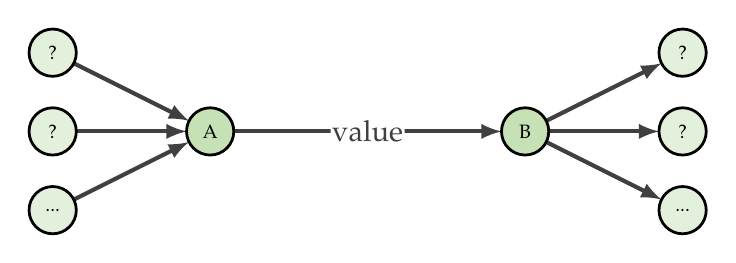
\begin{tikzpicture}
\Vertex[x=1,IdAsLabel=true,RGB,color={198, 225, 181}]{A}
\Vertex[x=5,IdAsLabel=true,RGB,color={198, 225, 181}]{B}
\Vertex[x=-1,y=1,label=?,RGB,color={227, 240, 219}]{X1}
\Vertex[x=-1,y=0,label=?,RGB,color={227, 240, 219}]{X2}
\Vertex[x=-1,y=-1,label=...,RGB,color={227, 240, 219}]{X3}
\Vertex[x=7,y=1,label=?,RGB,color={227, 240, 219}]{Y1}
\Vertex[x=7,y=0,label=?,RGB,color={227, 240, 219}]{Y2}
\Vertex[x=7,y=-1,label=...,RGB,color={227, 240, 219}]{Y3}
\Edge[Direct,label=value,fontscale=1.5](A)(B)
\Edge[Direct,fontscale=1](X1)(A)
\Edge[Direct,fontscale=1](X2)(A)
\Edge[Direct,fontscale=1](X3)(A)
\Edge[Direct,fontscale=1](B)(Y1)
\Edge[Direct,fontscale=1](B)(Y2)
\Edge[Direct,fontscale=1](B)(Y3)
\end{tikzpicture}
\caption{Weighted directed graph Model}\label{fig:networkstructure}
\end{figure}

On this basis, in order to explain the connection weight more specifically, let's take the relationship in the following Figure \ref{fig:different influence} as an example. Node A is the direct influencer of B, B is the direct influencer of CDE, and A is the indirect influencer of CDE. Next, we will analyze the musical characteristics of A and B. If the musical characteristics of A and B are similar, indicating that B is greatly affected by A, the indirect influence of A on CDE is greater as shown in Figure \ref{subfig:different influence left}. If the result is not similar, indicating that B is less affected by A, then A has a less indirect impact on CDE, as shown in Figure \ref{subfig:different influence right}. 

%图片2.1和2.2
\begin{figure}[htbp]
\centering
%图片2.1
\begin{subfigure}[b]{.4\textwidth}
\centering
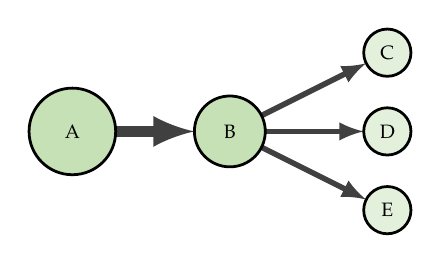
\begin{tikzpicture}
\Vertex[x=1,y=0,size=1.1,IdAsLabel=true,RGB,color={198, 225, 181}]{A}
\Vertex[x=3,y=0,size=0.9,IdAsLabel=true,RGB,color={198, 225, 181}]{B}
\Vertex[x=5,y=1,size=0.6,IdAsLabel=true,RGB,color={227, 240, 219}]{C}
\Vertex[x=5,y=0,size=0.6,IdAsLabel=true,RGB,color={227, 240, 219}]{D}
\Vertex[x=5,y=-1,size=0.6,IdAsLabel=true,RGB,color={227, 240, 219}]{E}
\Edge[Direct,lw=4](A)(B)
\Edge[Direct,lw=2](B)(C)
\Edge[Direct,lw=2](B)(D)
\Edge[Direct,lw=2](B)(E)
\end{tikzpicture}
\caption{Strong influence}\label{subfig:different influence left}
\end{subfigure}
%图片2.2
\begin{subfigure}[b]{.4\textwidth}
\centering
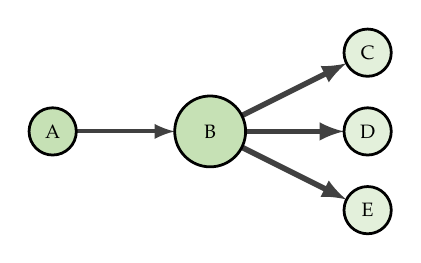
\begin{tikzpicture}
\Vertex[x=1,y=0,size=0.6,IdAsLabel=true,RGB,color={198, 225, 181}]{A}
\Vertex[x=3,y=0,size=0.9,IdAsLabel=true,RGB,color={198, 225, 181}]{B}
\Vertex[x=5,y=1,size=0.6,IdAsLabel=true,RGB,color={227, 240, 219}]{C}
\Vertex[x=5,y=0,size=0.6,IdAsLabel=true,RGB,color={227, 240, 219}]{D}
\Vertex[x=5,y=-1,size=0.6,IdAsLabel=true,RGB,color={227, 240, 219}]{E}
\Edge[Direct,lw=1.5](A)(B)
\Edge[Direct,lw=2](B)(C)
\Edge[Direct,lw=2](B)(D)
\Edge[Direct,lw=2](B)(E)
\end{tikzpicture}
\caption{Weak influence}\label{subfig:different influence right}
\end{subfigure}
\caption{Example of different influence}\label{fig:different influence}
\end{figure}
 
 In addition, the indirect impact should be smaller than the actual impact, so an attenuation factor $\alpha$ is introduced, and the final value is 0.2 through data comparison. Finally, the similarity between nodes are multiplied by the attenuation factor as the link weight, as shown in the Page \pageref{fig:weitghted} Figure \ref{fig:weitghted}. 
 
 %图片3[Weighted analysis diagram]
\begin{figure}[htbp]
\centering
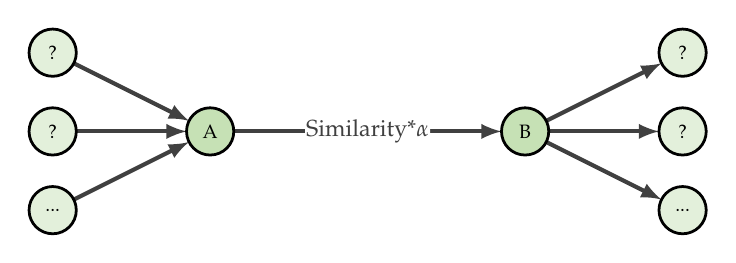
\begin{tikzpicture}
\Vertex[x=1,IdAsLabel=true,RGB,color={198, 225, 181}]{A}
\Vertex[x=5,IdAsLabel=true,RGB,color={198, 225, 181}]{B}
\Vertex[x=-1,y=1,label=?,RGB,color={227, 240, 219}]{X1}
\Vertex[x=-1,y=0,label=?,RGB,color={227, 240, 219}]{X2}
\Vertex[x=-1,y=-1,label=...,RGB,color={227, 240, 219}]{X3}
\Vertex[x=7,y=1,label=?,RGB,color={227, 240, 219}]{Y1}
\Vertex[x=7,y=0,label=?,RGB,color={227, 240, 219}]{Y2}
\Vertex[x=7,y=-1,label=...,RGB,color={227, 240, 219}]{Y3}
\Edge[Direct,label=Similarity*$\alpha$,fontscale=1.2](A)(B)
\Edge[Direct,fontscale=1](X1)(A)
\Edge[Direct,fontscale=1](X2)(A)
\Edge[Direct,fontscale=1](X3)(A)
\Edge[Direct,fontscale=1](B)(Y1)
\Edge[Direct,fontscale=1](B)(Y2)
\Edge[Direct,fontscale=1](B)(Y3)
\end{tikzpicture}
\caption{Weighted analysis diagram}\label{fig:weitghted}
\end{figure}
 
 
 
\subsubsection{Artists similarity measure}

From the $data$\_$by$\_$artist$ data set, the musical characteristics of each artist can be regarded as a multi-dimensional vector. The cosine similarity algorithm can evaluate the similarity of two vectors by calculating the cosine of the angle between them. Therefore, the cosine similarity algorithm can be used to calculate the similarity of the musical characteristics of two artists. The calculation formula is as Formula \ref{eq:cos}. 

%余弦相似度公式
\begin{equation}\label{eq:cos}
    cos\theta = \frac{\vec{a}\cdot \vec{b}}{\left \| \vec{a} \right \|\cdot \left \| \vec{b} \right \|}
\end{equation}

$\vec{a}$ and $\vec{b}$ are two multidimensional vectors. $\theta$ is the angle between the two vectors. 

Further, to solve the problem that the vector angle is too small and the vector length is very different, but the difference in the cosine value is small and the two vectors are judged to be similar, the modified cosine similarity algorithm is introduced, and the formula is as Formula \ref{eq:cosfix}.

%修正余弦公式
\begin{equation}\label{eq:cosfix}
    sim\left (  i,j\right )=\frac{\sum \left ( R_{ui} - \bar{R_u}\right ) \left ( R_{uj} - \bar{R_u}\right )}{\sqrt{\sum \left ( R_{ui} - \bar{R_u}\right )^{2}}\sqrt{\sum \left ( R_{uj} - \bar{R_u}\right )^{2}}}
\end{equation}

$i$ and $j$ are vector numbers. $R$ is a vector collection of multiple vectors. $R_{ui}$ represents the $u$-th dimension data of $i$ of the vector. $\bar{R_u}$ indicates the average value of the $u$-th dimension of all data.\par
Finally, since the value range of the cosine value is [-1, 1], we normalize the data obtained by the modified cosine similarity algorithm to obtain the final similarity measure between artists. The standardized formula is as Formula \ref{eq:standard formula}.

\begin{comment}

\ref{eq:yi} \ref{eq:barx} \ref{eq:s}.

\begin{equation}\label{eq:yi}
    y_i = \frac{x_i - \bar{x}}{s}  \\
\end{equation}

\begin{equation}\label{eq:barx}
    \bar{x}=\frac{1}{n}\sum_{i=1}^{n}x_i \\
\end{equation}

\begin{equation}\label{eq:s}
    s=\sqrt{\frac{1}{n-1}\sum_{i=1}^{n}\left ( x_i-\bar{x} \right )^{2}}\\
\end{equation}

$x_i$ is the data in the original data set, $s$ is the standard deviation of $x$, and $\bar{x}$ is the average value of the $x$ data set, $y_i$ is the normalized value of $x_i$. 
\end{comment}%标准化
\begin{equation}\label{eq:standard formula}
    y_i=\frac{x_i-min\{x_j\}}{max\{x_j\}-min\{x_j\}}
\end{equation}

$y_i$ is the normalized result of $x_i$. $x_i$ is the $i$-th component of the $x$ data set. 

\subsubsection{Network model supplement }

Based on the model above, there is no doubt that artists can influence their predecessors, but this part of the influence has a limited impetus to the development of music. To make the "music influence" parameter more realistic, that is, from the perspective of development, music development needs to be injected with fresh blood. Therefore, we define "music influence" as the "new generation talent influence", that is, the calculation of artist "music influence" includes only peer artists and younger artists. \par

In addition, due to the influence of music, the network contains loops. Based on our assumption, in the calculation of the influence of a single artist, there will be no situation that affects itself, so the loop is broken in the calculation of the single influence, which is shown in Figure \ref{fig:fixed networkstructure}. 

%避免回路的图像解释
\begin{figure}[htbp]
\centering
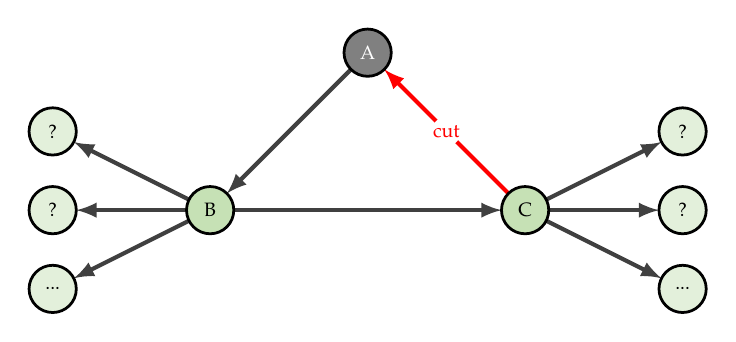
\begin{tikzpicture}
\Vertex[x=1,IdAsLabel=true,RGB,color={198, 225, 181}]{B}
\Vertex[x=5,IdAsLabel=true,RGB,color={198, 225, 181}]{C}
\Vertex[x=3,y=2,IdAsLabel=true,color=gray,fontcolor=white]{A}
\Vertex[x=-1,y=1,label=?,RGB,color={227, 240, 219}]{X1}
\Vertex[x=-1,y=0,label=?,RGB,color={227, 240, 219}]{X2}
\Vertex[x=-1,y=-1,label=...,RGB,color={227, 240, 219}]{X3}
\Vertex[x=7,y=1,label=?,RGB,color={227, 240, 219}]{Y1}
\Vertex[x=7,y=0,label=?,RGB,color={227, 240, 219}]{Y2}
\Vertex[x=7,y=-1,label=...,RGB,color={227, 240, 219}]{Y3}
\Edge[Direct](A)(B)
\Edge[Direct](B)(C)
\Edge[Direct,color=red,label=cut](C)(A)
\Edge[Direct](B)(X1)
\Edge[Direct](B)(X2)
\Edge[Direct](B)(X3)
\Edge[Direct](C)(Y1)
\Edge[Direct](C)(Y2)
\Edge[Direct](C)(Y3)
\end{tikzpicture}
\caption{Weighted directed graph Model}\label{fig:fixed networkstructure}
\end{figure}

\subsubsection{Music influence}

Combining the above content, we can finally get the recursive relationship of influence as Formula \ref{eq:recursive}.

\begin{equation}\label{eq:recursive}
    P_i = k+\alpha \sum_{j=1}^{k}P_{i_j}O_{i{i_j}}
\end{equation}

$P_i$ is the music influence parameter of the artist corresponding to the $i$-th node. $k$ is the number of child nodes directly connected to the $i$-th node. $\alpha$ is the attenuation factor. $P_{i_j}$ is the music influence parameter of the corresponding artist of the $j$-th directly connected child node of the $i$-th node. $O_{i_j}$ is the similarity of music characteristics between the artist corresponding to the $i$-th node and the artist corresponding to the $j$-th directly connected child node. \par


In the network we have established, "music influence" which is the same thing as "new generation talent influence" can be used to reveal which music masters in the genre and the proportion of music masters in each genre. Thus, we select the top five "music influence" artists of the genre as masters in the following Page \pageref{tab:Top 5 Influencers} Table \ref{tab:Top 5 Influencers}, and analyze the top 500 music influence artists to draw the image as shown in Page \pageref{fig:top500} Figure \ref{fig:top500}.

%影响力排行前5的音乐家表格
\begin{table}[htbp]
\caption{Top 5 Influencers}
\label{tab:Top 5 Influencers}
\centering
\begin{tabular}{llll}
\hline\hline
\rowcolor[rgb]{0.663, 0.816, 0.557}name               & influence & genre    & year \\ \hline
\rowcolor[rgb]{0.886, 0.937, 0.855} The Beatles        & 790.9253  & Pop/Rock & 1960 \\
Bob Dylan          & 523.7476  & Pop/Rock & 1960 \\
\rowcolor[rgb]{0.886, 0.937, 0.855} Hank Williams      & 451.7476  & Country  & 1930 \\
The Rolling Stones & 434.6987  & Pop/Rock & 1960 \\
\rowcolor[rgb]{0.886, 0.937, 0.855} David Bowie        & 416.7795  & Pop/Rock & 1960 \\ \hline\hline
\end{tabular}
\end{table}

%top500音乐家的流派分布
\begin{figure}[htbp]
\centering
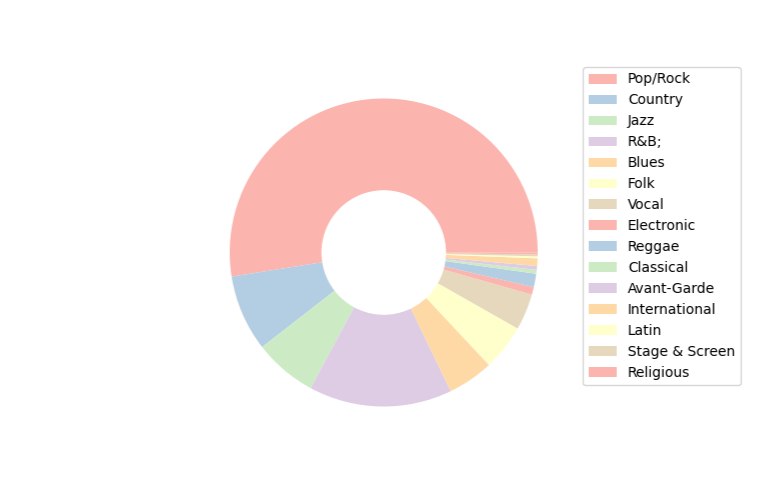
\includegraphics[width=.8\textwidth]{TOP500.png}
\caption{Top 500 Influencers}\label{fig:top500}
\end{figure}

\subsubsection{Artists similarity comparison}

Let us take the pop/rock genre as an example. We first calculate the modified cosine similarity for every two artists in the genre, and get the average similarity in the pop/rock genre by summing and averaging. Then we calculate the similarity of any two artists in the network, and average the sum.

%对相似度进行求和取平均的公式

\begin{equation}
    \bar{O}=\frac{\sum_{i}^{n}\sum_{j}^{n}O_i_j }{\frac{1}{2}n\left ( n-1 \right )}\left ( 1\leq i< j \leq n\right )
\end{equation}

$\bar{O}$ is the average similarity of artists. $O_{ij}$ is the similarity of the music characteristics of the artist corresponding to node $i$ and the artist corresponding to node $j$.  $n$ is the number of all nodes.\par

Finally, we get the average similarity of artists in the pop/rock genre and the overall average similarity of artists as Page \pageref{fig:Pop Similarity} Figure \ref{fig:Pop Similarity}. 

%Pop/Rock内部相似度与全部平均相似度比较
\begin{figure}[htbp]
\centering
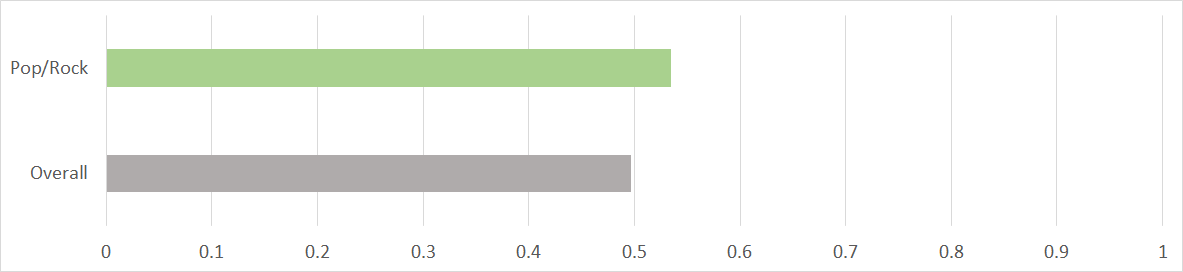
\includegraphics[width=.9\textwidth]{img/Pop Similarity.jpg}
\caption{Similarity Comparision (Pop/Rock)}\label{fig:Pop Similarity}
\end{figure}

By analyzing the figure, we can see that the average artist similarity of the pop/
rock genre is higher than the overall average similarity, that is, the artists within the pop/rock genre are more similar.


\subsection{Genre Analysis }

In the analysis of different genres, artists who do not know the genre will not participate in the genre analysis, that is, the genre “$unknown$” will not participate in the analysis. 

\subsubsection{Inter-genre analysis }

We separately sum the music characteristics of all artists in each genre that have been preprocessed and get the average music characteristics of each genre. Perform modified cosine similarity calculation for different genres, and finally perform normalization. The following Table \ref{tab:Similarity between genres} shows part of our result.

%流派间相似度表格
\begin{table}[htbp]
\centering
\caption{Table of Similarity between genres}
\label{tab:Similarity between genres}
\begin{tabular}{l|lllllll}
                                                       & Pop/Rock & Country  & Jazz     & R\&B;    & Blues    & Folk     & ... \\ \hline
Pop/Rock                                               & NULL     & 0.383519 & 0.066974 & 0.390405 & 0.074175 & 0.081382 & ... \\
\cellcolor[HTML]{FFFFFF}{\color[HTML]{333333} Country} & NULL     & NULL     & 0.407583 & 0.618256 & 0.81085  & 0.757632 & ... \\
Jazz                                                   & NULL     & NULL     & NULL     & 0.359063 & 0.793443 & 0.831264 & ... \\
R\&B;                                                  & NULL     & NULL     & NULL     & NULL     & 0.577393 & 0.395399 & ... \\
Blues                                                  & NULL     & NULL     & NULL     & NULL     & NULL     & 0.926958 & ... \\
Folk                                                   & NULL     & NULL     & NULL     & NULL     & NULL     & NULL     & ... \\
...                                                    & ...      & ...      & ...      & ...      & ...      & ...      & ...
\end{tabular}
\end{table}

We analyze the music characteristics of the two genres with the lowest similarity, namely Pop/Rock-International, and it is shown that almost all the characteristics of these two genres in Table \ref{tab:characteristics of Pop/Rock and International} are distributed on the upper and lower sides of the average line respectively, which can be considered as opposite. It is also shown that the similarity between Avant-Garde and New Age is "1"(relative value), so it can be considered that these two genres are related to a certain extent. 

\begin{table}[htbp]
\caption{The average characteristics of Pop/Rock and International}
\label{tab:characteristics of Pop/Rock and International}
\begin{tabular}{l|lllll}
           & danceability & energy       & valence      & tempo            & loudness \\ \hline
Pop/Rock   & -0.22646     & 0.433394     & -0.0851      & 0.203152         & 0.31915  \\
International & 0.092088     & -0.55538     & 0.274276     & -0.27295         & -0.52357 \\ \hline
           & mode         & key          & acousticness & instrumentalness & liveness \\ \hline
Pop/Rock   & 0.105595     & 0.015097     & -0.44957     & -0.11148         & 0.04429  \\
International     & -0.0492      & -0.04414     & 0.843321     & 0.04737          & -0.09579 \\ \hline
            & speechiness  & duration\_ms & popularity   &                  &          \\ \hline
Pop/Rock   & -0.1031      & -0.08031     & 0.252042     &                  &          \\
International   & 0.063525     & 0.364976     & -0.38035     &                  &
\end{tabular}
\end{table}

Next, we use the music influence network to calculate the "music influence" of each artist and sum up the musical influence of artists in each genre to obtain the musical influence of the genre.

%各流派总影响力
\begin{figure}[htbp]
\centering
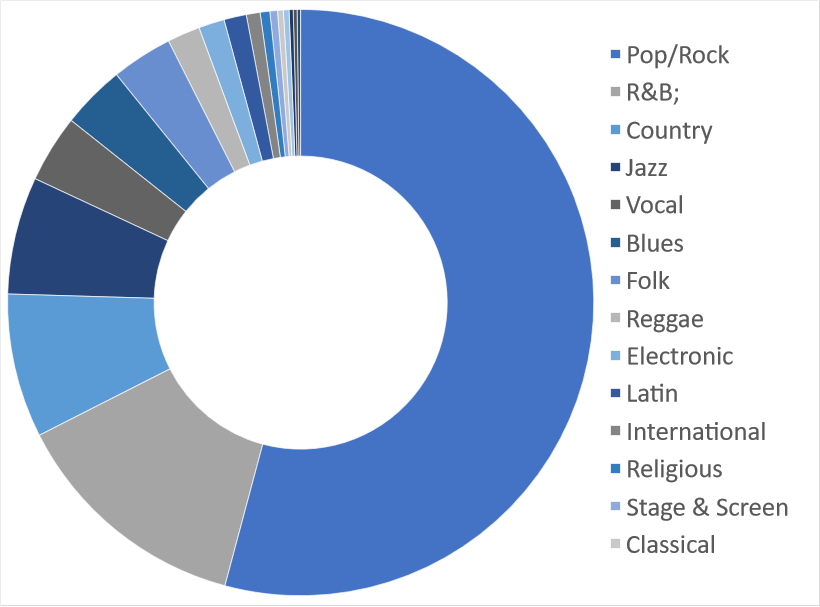
\includegraphics[width=.7\textwidth]{img/Genre Influence.jpg}
\caption{Genre Music Influence}\label{fig:Genre Influence}
\end{figure}

From the Figure \ref{fig:Genre Influence}, it can be concluded that pop/rock, R\&B and country are the three genres with the highest "music influence", among which the "music influence" of the pop/rock genre far exceeds other genres, indicating that the pop/rock genre attracts the newest talents and the most popular and developing best. 


\subsubsection{Genre internal analysis }

We calculate the similarity of every two artists within each genre and take the average to get the average internal similarity of each genre, as shown in the following Figure \ref{fig:Internal similarity table of genres} in Page  \pageref{fig:Internal similarity table of genres}.

\begin{figure}[htbp]
\centering
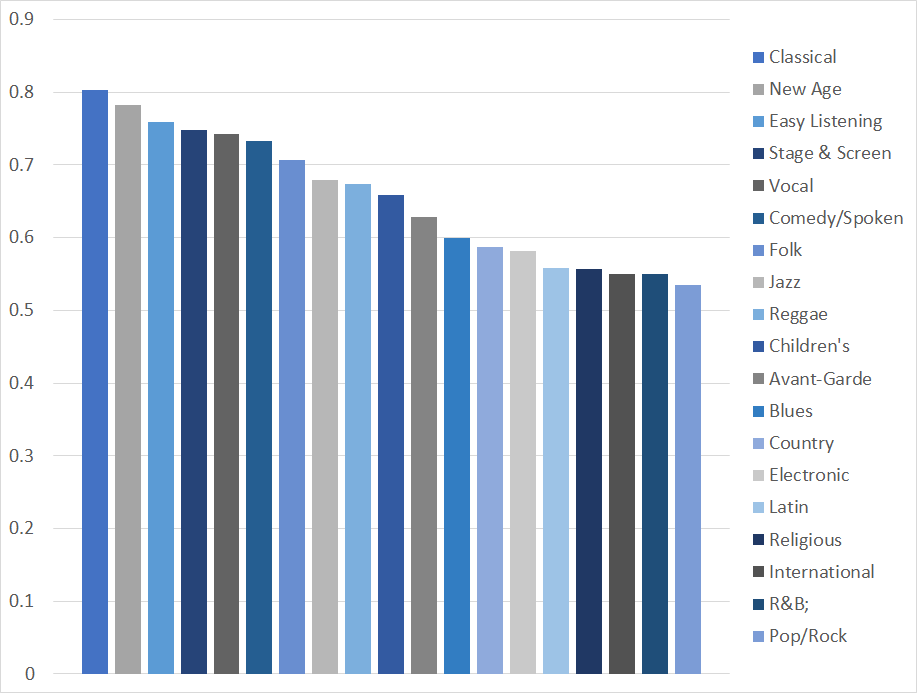
\includegraphics[width=.7\textwidth]{img/Genre Similarity.jpg}
\caption{Internal similarity of genres}\label{fig:Internal similarity table of genres}
\end{figure}

From the Figure \ref{fig:Internal similarity table of genres}, it can be known that Classical, New Age and Easy Listening are the three most similar genres, indicating that the music characteristics of different artists within these genres are similar. Similarly, pop/rock, R\&B and international are the three genres with the lowest similarity, which indicates that different artists within these genres have diverse styles and a high degree of discreetness in music characteristics. 


\subsubsection{Popular genres change over time }

According to the hypothesis, through the data by artist data set, we can get the time when every artist started to be active, and use this to determine that the musical characteristics of every artist only contributed to their respective decade. Average the musical characteristics of artists in each genre that have been active in each decade (10 years), and obtain the average musical characteristics of each genre per decade. Next, we obtain the overall average music characteristics of all genres per decade in the data by year data set. By analyzing the similarity between the average music characteristics of each genre and the average music characteristics of the decade, we can find the genre with the highest similarity in every decade. According to the hypothesis, it can be considered that this genre is the most popular in that decade. Popular genres change over time as shown in the Table \ref{tab:Popular genre}.

%逐年最流行的流派
\begin{table}[htbp]
\centering
\caption{Popular genres by year}
\label{tab:Popular genre}
\begin{tabular}{l|lllll}
Rank & 1930       & 1940          & 1950     & 1960          & 1970          \\ \hline
1    & Jazz       & International & Blues    & Folk          & R\&B;         \\
2    & Vocal      & Vocal         & Folk     & Country       & International \\
3    & Folk       & Jazz          & Country  & International & Blues         \\ \hline
Rank & 1980       & 1990          & 2000     & 2010          &               \\ \hline
1    & Pop/Rock   & Pop/Rock      & Pop/Rock & Pop/Rock      &               \\
2    & Electronic & Religious     & Country  & Electronic    &               \\
3    & Unknown    & Country       & R\&B;    & R\&B;         &              \end{tabular}
\end{table}

It can be seen form the table that from 1930 to 1979, Jazz, International, Blues, Folk, Vocal and Country all took turns occupying the top three influential lists. But after 1980, Pop/Rock ranked first in the influence list by absolute advantage.


\subsection{Influencer's Music Influence Analysis }

In Figure \ref{fig:Pop Similarity} we have obtained the overall average similarity. Based on this, we found that the average similarity between artists with mutual influence in the network, as shown in the following Figure \ref{fig:Overall vs Node to node}.

%[Influencer influence analysis table]
\begin{figure}[htbp]
\centering
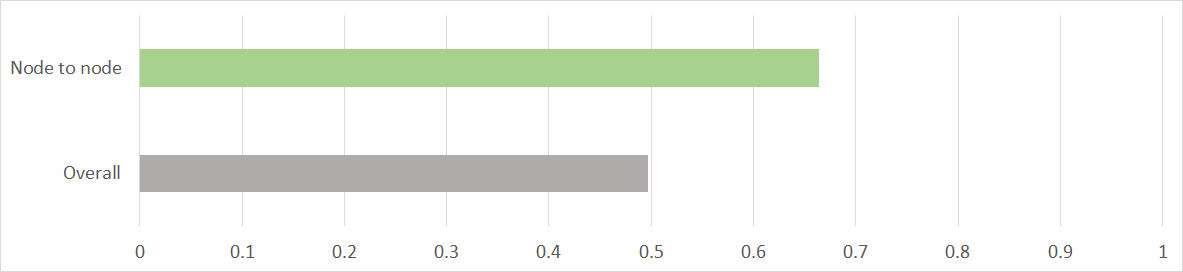
\includegraphics[width=.7\textwidth]{img/Overall vs Node to node.jpg}
\caption{Similarity between artists with mutual influence}\label{fig:Overall vs Node to node}
\end{figure}

From the greater average similarity of directly influencing artists, it can be known that "influencers" will affect the music created by followers, and followers will learn the music styles of influencers, and they have more similarities. \par

To further determine the music characteristics affected by followers, the Pearson correlation coefficient algorithm is used to determine the relationship between the influencers’ and the followers’ music characteristics, which is determined by the following Formula  \ref{eq:piersen}.


\begin{equation}\label{eq:piersen}
    \rho_{U,V}=\frac{\sum UV-\frac{\sum U\sum V}{N}}{\sqrt{\left ( \sum U^{2}-\frac{\left ( \sum U \right )^{2}}{N} \right )\left ( \sum V^{2}-\frac{\left ( \sum V \right )^{2}}{N} \right )}}
\end{equation}

$U$ and $V$ represent data sets, and the elements between them have a one-to-one correspondence. $N$ is the total number of corresponding element pairs in $U$ and $V$. If $U$ and $V$ are highly correlated, the Pearson correlation coefficient tends to 1, otherwise, it tends to 0. \par

In the network, we take the 13 music characteristics of the influencer as $U$ and the corresponding music characteristic of the affected person as $V$, and obtain the two-dimensional data ($U$, $V$) of 13 sets of music characteristics, and then calculate the data of each group of music characteristics. Pearson correlation coefficient, the Pearson correlation coefficient of 13 music characteristics is obtained, and the histogram is drawn as Figure \ref{fig:Pearson}.

%[Pearson's correlation coefficient histogram]
\begin{figure}[htbp]
\centering
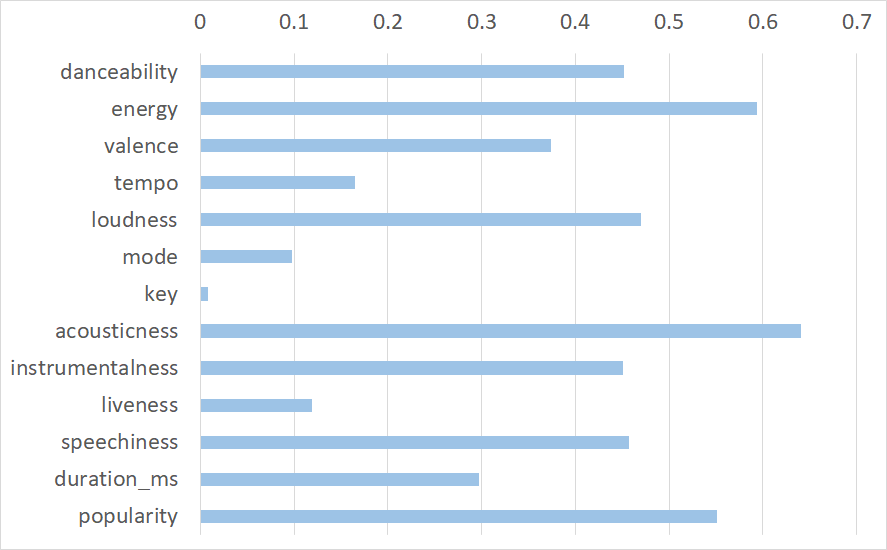
\includegraphics[width=.7\textwidth]{img/Pearson.jpg}
\caption{Pearson's correlation coefficient histogram}\label{fig:Pearson}
\end{figure}

Analyzing the histogram in Figure \ref{fig:Pearson}, we can find that the Pearson coefficients of these two musical characteristics are very prominent, which means that they are highly transmissible in the influence network.





\subsection{Music Revolution Analysis}

First, we perform year-by-year similarity calculation on the music characteristics of the data by year data set, and calculate the music similarity between each adjacent two years, as shown in the following Figure \ref{fig:Yearly Music Similarity}. 

%[Yearly Music Similarity]
\begin{figure}[htbp]
\centering
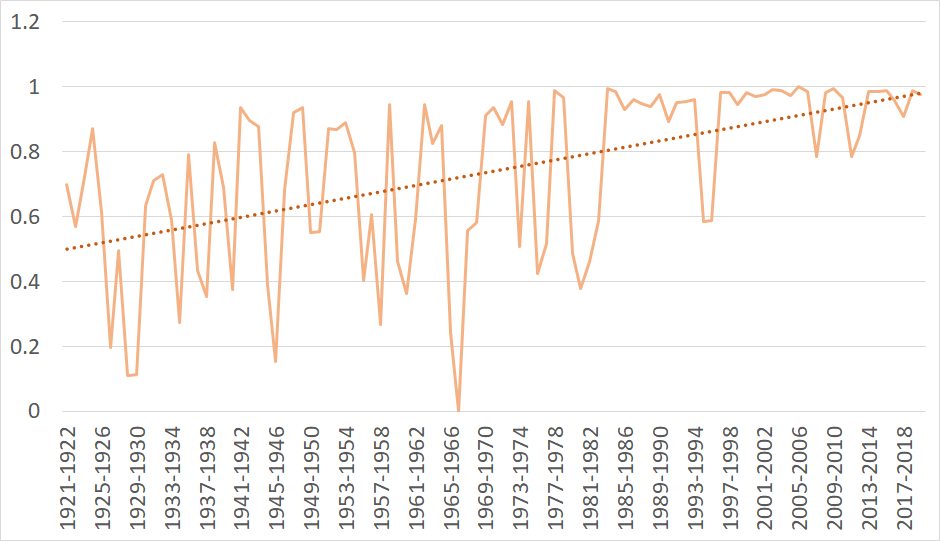
\includegraphics[width=.7\textwidth]{img/Similarity year by year.jpg}
\caption{Yearly Music Similarity}\label{fig:Yearly Music Similarity}
\end{figure}


As can be seen from the figure, the similarity of music characteristics of 1929, 1945, 1967 and 1981 with those of the previous year is the lowest, indicating that some of these years have great changes in music characteristics and may have undergone musical changes. Next, we look for artists whose music has a strong influence on the network and whose music features are highly similar to those of the years of change. Then the artists that are eventually found can be considered as musical revolutionaries.\par


Taking 1967 as an example, we found that The Beatles, The Rolling Stones and David Bowie had a great influence, and their similarity with that year's music features reached 0.9. Therefore, it is believed that they are revolutionaries of the 1967 music revolution.


\subsection{Pop/Rock Genre Analysis}

The entropy weight method(EWM) can use the entropy value to judge the degree of dispersion of an index. The smaller the information entropy value, the greater the degree of dispersion of the index. By calculating the entropy value of each music feature, the dynamic influence index can be obtained. \par

If there are $l$ $X_i$ data sets, $X_{ij}$ ($i$ < $l$, $j$ < $n$)represents the $j$-th element in the $i$-th data set. We use formula \ref{eq:standard formula} to normalize $X_i$ to get the $l$ normalized data set $Y_i$.

\begin{equation}\label{eq:xdataset}
    X_i = \{ x_1,x_2,...,x_n\}
\end{equation}



We define standardized treatment for $Y_{ij}$ as in formula \ref{eq:Ystandard}. $p_{ij}$ is the normalized result of $Y_{ij}$.

\begin{equation}\label{eq:Ystandard}
    p_{ij}=\frac{Y{ij}}{\sum_{i=1}^{l}Y_{ij}}
\end{equation}

If $p_{ij}$=0, then $\lim_{p_{ij}\rightarrow 0} p_{ij}lnp_{ij}=0$.

For the information entropy E of a set of data, we can obtain the following Formula \ref{eq:E}.

\begin{equation}\label{eq:E}
    E_j=-\frac{1}{ln l}\sum_{i=1}^{l}p_{ij}lnp_{ij}
\end{equation}

Finally, we can calculate the weight of each indicator through information entropy, as shown in Formula \ref{eq:quanzhong}. If the weight of the index is large, it means that the index has a high entropy weight, a high degree of dispersion, and is unstable. If the weight is small, the entropy weight is small and the index is relatively stable. 

\begin{equation}\label{eq:quanzhong}
    W_i = \frac{1-E_i}{l-\sum E_i}\left ( i=1,2,...,l \right )
\end{equation}


We calculated the average music characteristics of pop/rock each year in the full music data data set, using 10 years as an interval, and using the entropy method to calculate the change weights of music characteristics within ten years. The greater the weight of the music characteristics, the greater the value of the music characteristics. The greater the degree of dispersion within ten years, the greater the dynamic impact. Keep the first three entropy values of every ten years, the output table is as follows.

%[Top three characteristics of entropy method]
\begin{table}[htbp]
\small
\centering
\caption{Top three characteristics of entropy method}
\label{tab:Entropy method data}
\begin{tabular}{l|lll}
     & No.1             & No.2             & No.3         \\ \hline
1940 & energy           & valence          & tempo        \\
1950 & speechiness      & instrumentalness & energy       \\
1960 & duration\_ms     & danceability     & valence      \\
1970 & valence          & loudness         & liveness     \\
1980 & liveness         & loudness         & tempo        \\
1990 & instrumentalness & speechiness      & loudness     \\
2000 & valence          & loudness         & liveness     \\
2010 & liveness         & duration\_ms     & energy
\end{tabular}
\end{table}

It can be seen from Table \ref{tab:Entropy method data} in Page \pageref{tab:Entropy method data} that the valence, liveness and loudness music characteristics of the pop/rock genre have been in the region of high entropy weight for the past 70 years, that is, dynamic music characteristics with greater volatility. These musical characteristics are indicators that reflect the dynamic changes of music. Standardize the four music characteristics and draw the image as shown in Page \pageref{fig:changeovertime} Figure \ref{fig:changeovertime}. It can be seen that in the 1940s and 1950s, the pop/rock genre was still in the groping stage, and the genre music characteristics changed greatly. After the 1960s, the energy and loudness music characteristics were taken as examples. They showed an overall upward trend over time. The loudness and activity of pop/rock is getting bigger and bigger. 

\begin{figure}[htbp]
\centering
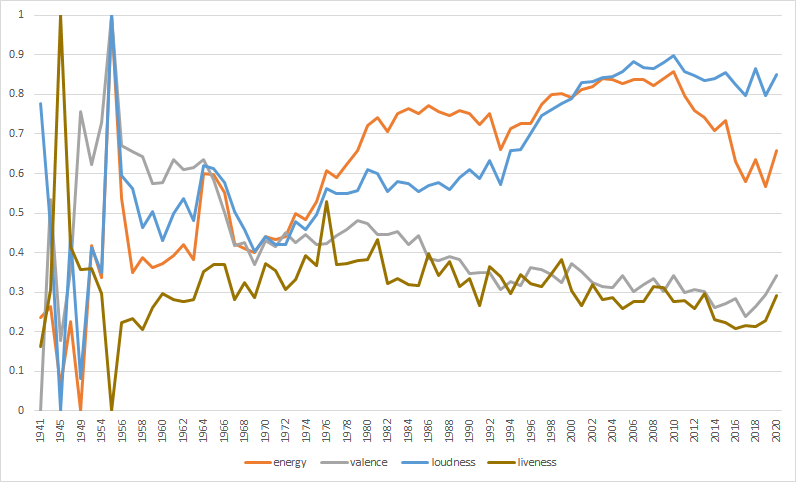
\includegraphics[width=.8\textwidth]{Simi by year.png}
\caption{Pop/Rock Music characteristics change over time}\label{fig:changeovertime}
\end{figure}

\subsection{The relationship between music and culture}


To explore the relationship between music and culture, it is natural to discuss the influence of music on culture and the reflection of music on social changes. The following details the main ideas of using the influence network model constructed by our group to analyze the above two relationships. 

\subsubsection{The impact of music on culture }

To get the main influence of music on culture in a particular era, we need to explore the corresponding era subnet of the influence network. First, search for several artists with high influence (five artists for example) and list them in the form of a table. Analyzing their genres and musical styles, and combining historical events, we can know where the main influence of music on culture in this era is reflected. 

\subsubsection{Music reflects cultural changes}

The music itself is constantly changing and evolving. This process is slow and stable. But in some cases, major external events can make music a great leap and improve. To illustrate the idea of identifying external influences, we might as well take the Pop/Rock genre as an example for analysis, and the same is true for the analysis of external influences that cause changes in all music genres.\par

In order to get the music changes that occurred in a certain period, we use the key music characteristics obtained through the entropy method in 4.6 to analyze. The size and change trend of these selected music characteristics are comprehensively analyzed to finally identify external influences. Take 2000s for example, the top three dramatic musical characteristics of the changes are valence, loudness and liveness. The trends of these three musical characteristics of Pop/Rock in the 2000s can be found in the Figure \ref{fig:Three characteristics of Pop/Rock} in Page \pageref{fig:Three characteristics of Pop/Rock}. 

%[Three main musical characteristics of Pop/Rock]
\begin{figure}[htbp]
\centering
\begin{subfigure}[b]{.7\textwidth}
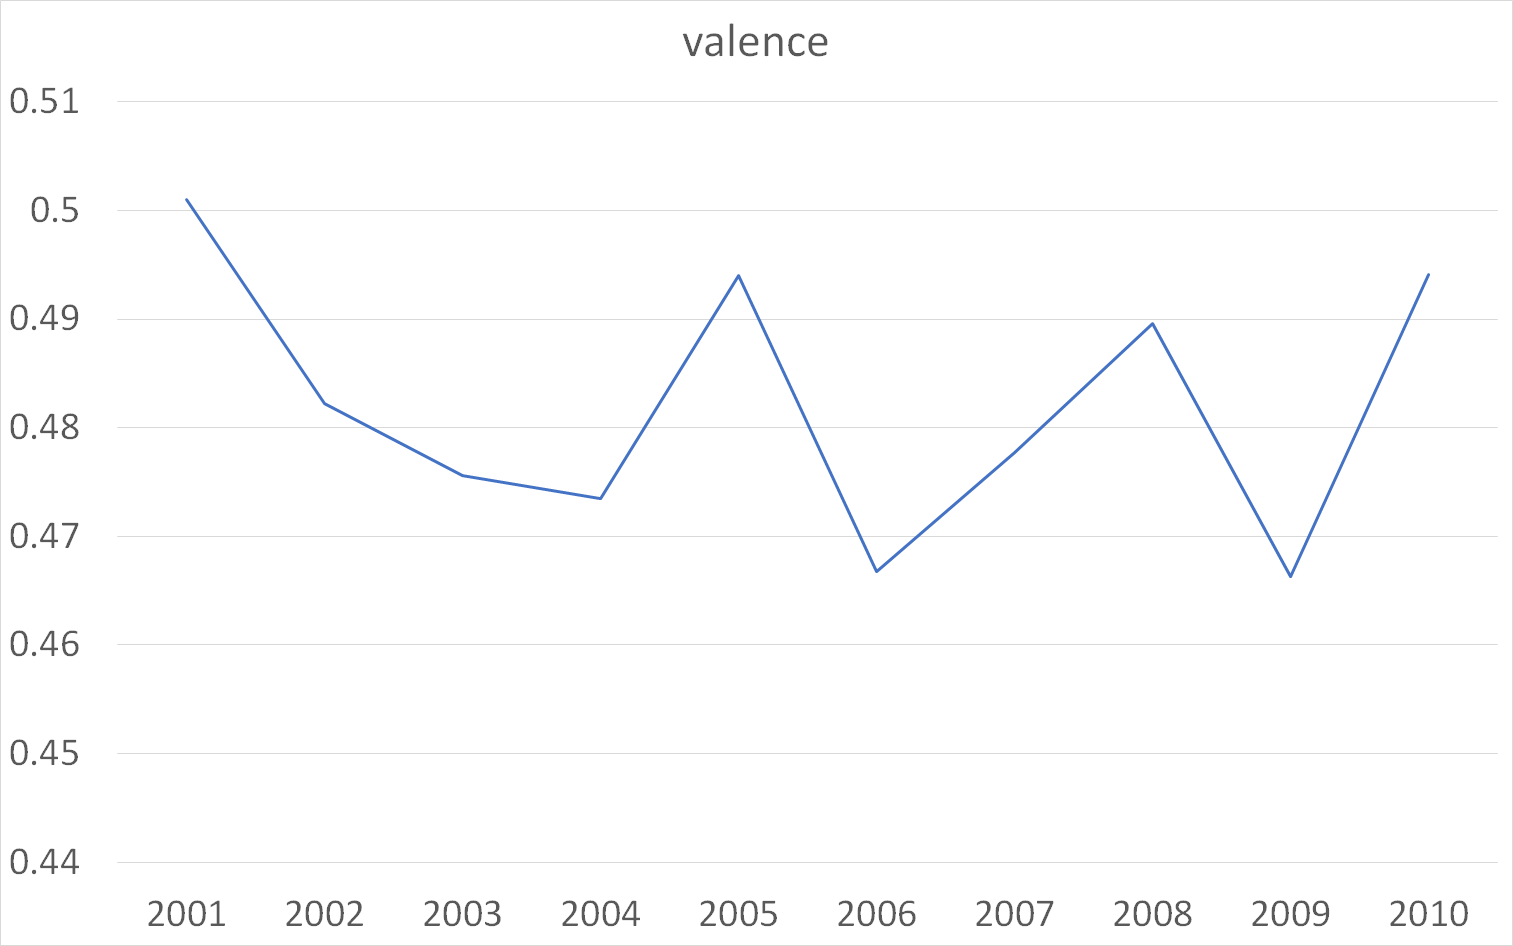
\includegraphics[width=\textwidth]{img/valence.jpg}
\caption{valence}\label{subfig:valence}
\end{subfigure}
\begin{subfigure}[b]{.7\textwidth}
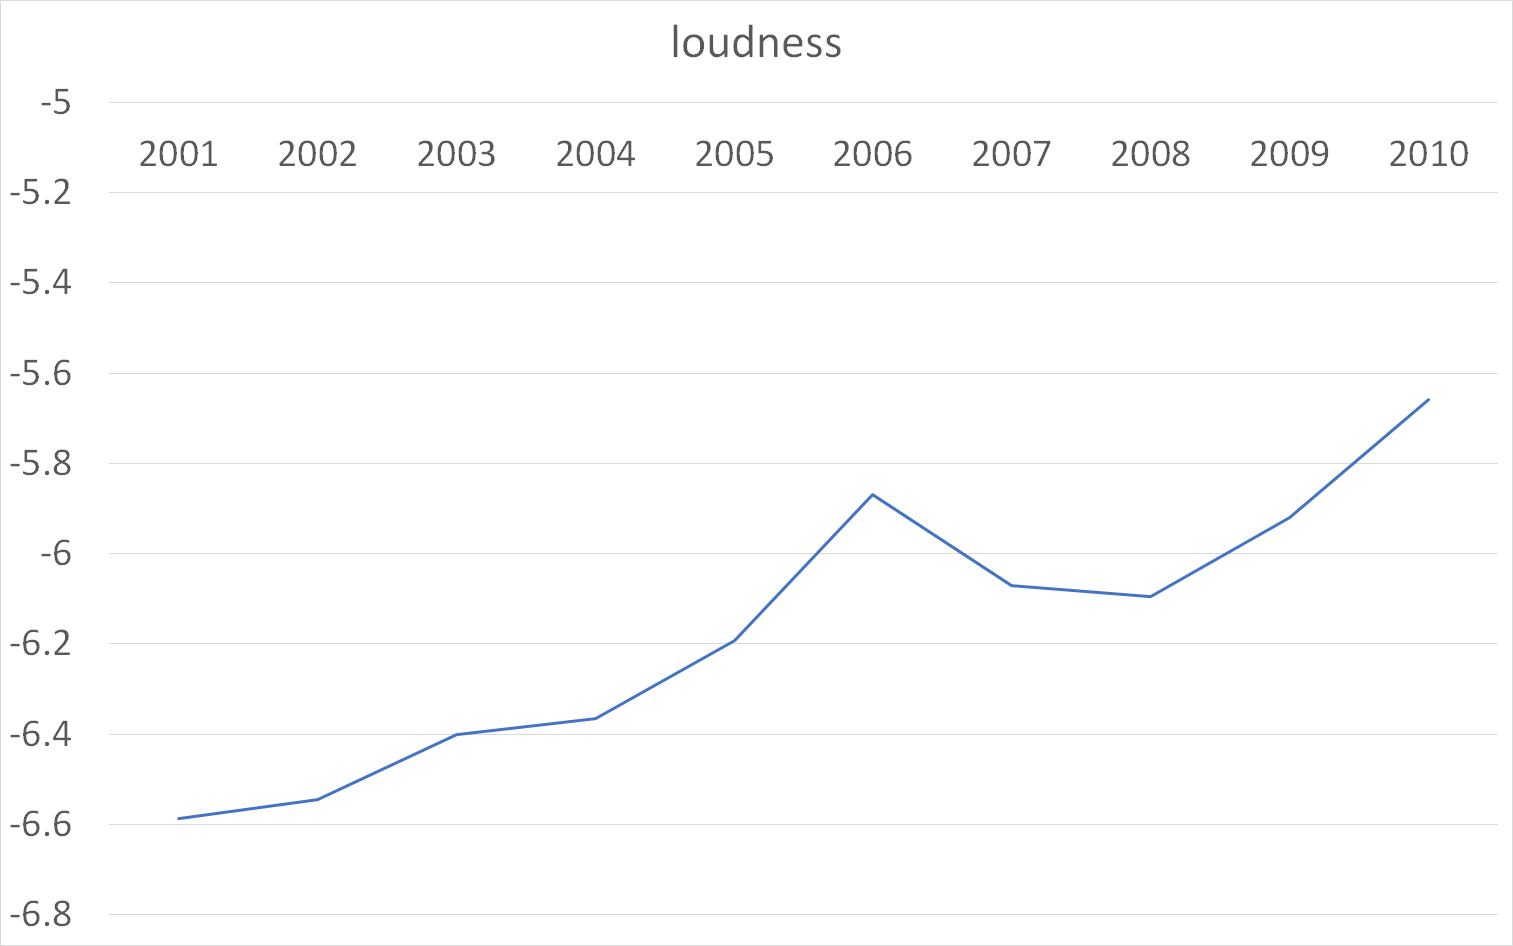
\includegraphics[width=\textwidth]{img/loudness.jpg}
\caption{loudness}\label{subfig:loudness}
\end{subfigure}
\begin{subfigure}[b]{.7\textwidth}
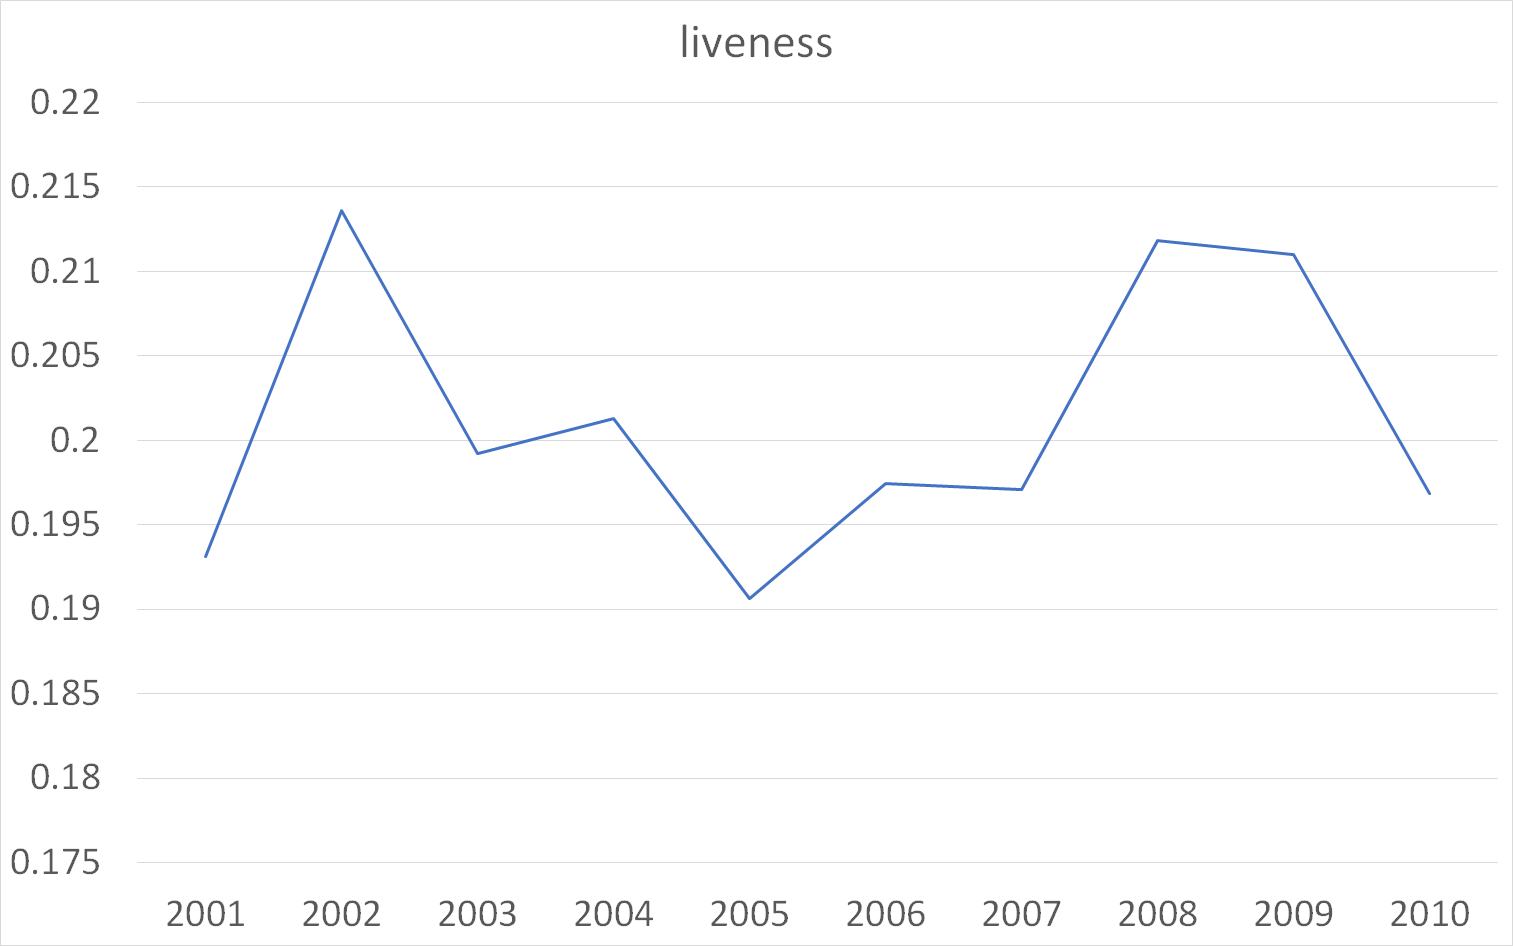
\includegraphics[width=\textwidth]{img/liveness.jpg}
\caption{liveness}\label{subfig:liveness}
\end{subfigure}
\caption{Three main musical characteristics of Pop/Rock}\label{fig:Three characteristics of Pop/Rock}
\end{figure}


Among them, the trend of the loudness curve can be clearly found. After the 1980s, the popularization of digital technology turned into a wave of economic growth in the 21st century. The spread of commercial music has continued to increase, and the people's economic purchasing power in some countries has also grown steadily.\cite{held_globalizing_2004} In addition, studies have shown that under the multiple influence of listener preferences and human instincts, louder music can achieve better sales in the world music market. This phenomenon is also called "loudness war".\cite{vickers_loudness_2011} Combining academic analysis articles and historical facts of other music, the sudden increase in loudness reflects the dual impact of the advancement of digital technology and economic globalization.


\begin{comment}%注释开始

%\subsubsection{Details about Model 1}
%The detail can be described by equation \eqref{eq:heat}:
%\begin{equation}\label{eq:heat}
%\frac{\partial u}{\partial t} - a^2 \left( \frac{\partial^2 u}{\partial x^2} + %\frac{\partial^2 u}{\partial y^2} + \frac{\partial^2 u}{\partial z^2} \right) = f(x, %y, z, t)
%\end{equation}

%\subsection{Model 2}
%\subsubsection{Conclusion of Model 2}
%The results are shown in Figure \ref{fig:result}, where $t$ denotes the time in %seconds, and $c$ refers to the concentration of water in the boiler.

%\begin{figure}[htbp]
%\centering
%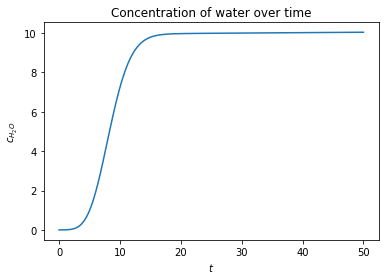
\includegraphics[width=.6\textwidth]{water.png}
%\caption{The result of Model 2}\label{fig:result}
%\end{figure}

%\subsubsection{Commetary on Model 2}
%The instance of long and wide tables are shown in Table \ref{tb:longtable}.

% 长表格示例,更多用法请参考 longtable 宏包文档
% 以下环境及对应参数可实现表格内的自动换行与表格的自动断页
% 您也可以选择自行载入 tabularx 宏包,并通过 X 参数指定对应列自动换行
\begin{longtable}{ p{4em} p{14em} p{14em} }
%\caption{Basic Information about Three Main Continents (scratched from Wikipedia)}
%\label{tb:longtable}\\
%\toprule
%Continent & Description & Information \\
%\midrule
%Africa & Africa Continent is surrounded by the Mediterranean Sea to the
%north, the Isthmus of Suez and the Red Sea to the northeast, the Indian
%Ocean to the southeast and the Atlantic Ocean to the west. &
%At about 30.3 million km$^2$ including adjacent islands, it covers 6\%
%of Earth's total surface area and 20\% of its land area. With 1.3
%billion people as of 2018, it accounts for about 16\% of the world's
%human population. \\
%\midrule
%Asia & Asia is Earth's largest and most populous continent which
%located primarily in the Eastern and Northern Hemispheres.


It shares the continental landmass of Eurasia with the continent
of Europe and the continental landmass of Afro-Eurasia with both
Europe and Africa. &
Asia covers an area of 44,579,000 square kilometers, about 30\%
of Earth's total land area and 8.7\% of the Earth's total surface
area. Its 4.5 billion people (as of June 2019) constitute roughly
60\% of the world's population. \\
\midrule
Europe & Europe is a continent located entirely in the Northern
Hemisphere and mostly in the Eastern Hemisphere. It comprises the
westernmost part of Eurasia and is bordered by the Arctic Ocean to
the north, the Atlantic Ocean to the west, the Mediterranean Sea to
the south, and Asia to the east. &
Europe covers about 10,180,000 km$^2$, or 2\% of the Earth's surface
(6.8\% of land area), making it the second-smallest
continent. Europe had a total population of about 741 million (about
11\% of the world population) as of 2018. \\
\bottomrule
\end{longtable}

Figure \ref{fig:subfigures} gives an example of subfigures. Figure \ref{subfig:left} is on the left, and Figure \ref{subfig:right} is on the right.

% 子图(多图并列)示例,更多用法请参考 subfigure 宏包文档
% 如果您只希望几张图并列,不需要额外的 caption,那么在 figure 环境中
% 连续插入总宽度不超过 \textwidth 的多个 \includegraphics 命令即可
\begin{figure}[htbp]
\centering
\begin{subfigure}[b]{.4\textwidth}
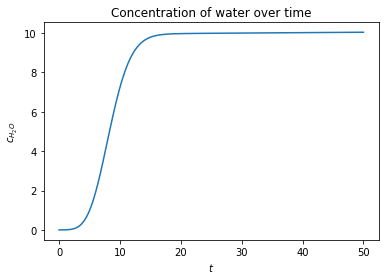
\includegraphics[width=\textwidth]{water.png}
\caption{Image on the left}\label{subfig:left}
\end{subfigure}
\begin{subfigure}[b]{.4\textwidth}
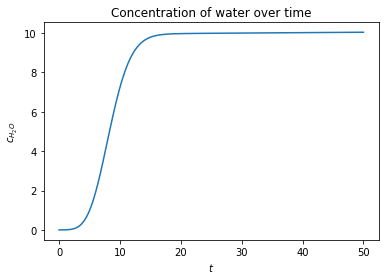
\includegraphics[width=\textwidth]{water.png}
\caption{Image on the right}\label{subfig:right}
\end{subfigure}
\caption{Two images}\label{fig:subfigures}
\end{figure}

\end{comment}%注释结束

\section{Model Evaluation}
\subsection{Model stability analysis}

We conduct stability analysis on the main model established, namely the music influence model. It can be seen that we initially set the attenuation factor $\alpha$ to 0.2. In order to explore the impact of changing the attenuation factor on the model results, output the top 20 "music influence" artists when the attenuation factor is 0.2, and then adjust the attenuation factor to 0.1 and output the first two Ten "music influence" artists. The data are shown in Tables \ref{tab:top20} and  \ref{tab:Top20} below.


\begin{minipage}{\textwidth}
 \begin{minipage}[t]{0.45\textwidth}
  \centering
     \makeatletter\def\@captype{table}\makeatother\caption{Top 20 Influencers by \alpha=0.1}\label{tab:top20}
       \begin{tabular}{ll} 
            \hline\hline
            \rowcolor[rgb]{0.663, 0.816, 0.557}name                   & influence \\
            \hline
            \rowcolor[rgb]{0.886, 0.937, 0.855}The Beatles            & 693.22 \\
            Bob Dylan              & 445.13    \\
            \rowcolor[rgb]{0.886, 0.937, 0.855}The Rolling Stones     & 371.14 \\
            David Bowie            & 316.27  \\
            \rowcolor[rgb]{0.886, 0.937, 0.855}Hank Williams          & 297.41  \\
            Led Zeppelin           & 279.41  \\
            \rowcolor[rgb]{0.886, 0.937, 0.855}The Kinks              & 256.32   \\
            Chuck Berry            & 240.96  \\
            \rowcolor[rgb]{0.886, 0.937, 0.855}Jimi Hendrix           & 237.81 \\
            The Velvet Underground & 236.58  \\
            \rowcolor[rgb]{0.886, 0.937, 0.855}Elvis Presley          & 233.57  \\
            Sex Pistols            & 224.98  \\
            \rowcolor[rgb]{0.886, 0.937, 0.855}Black Sabbath          & 215.77 \\
            Pink Floyd             & 210.99  \\
            \rowcolor[rgb]{0.886, 0.937, 0.855}The Beach Boys         & 209.90  \\
            Miles Davis            & 209.70  \\
            \rowcolor[rgb]{0.886, 0.937, 0.855}The Clash              & 204.51   \\
            Marvin Gaye            & 200.16 \\
            \rowcolor[rgb]{0.886, 0.937, 0.855}James Brown            & 198.91 \\
            The Who           & 194.02 \\
            \hline\hline
    \end{tabular}
  \end{minipage}
  \begin{minipage}[t]{0.45\textwidth}
   \centering
        \makeatletter\def\@captype{table}\makeatother\caption{Top 20 Influencers by \alpha=0.2}\label{tab:Top20}
         \begin{tabular}{ll}        
            \hline\hline
            \rowcolor[rgb]{0.663, 0.816, 0.557}{name}          & influence \\
            \hline
            \rowcolor[rgb]{0.886, 0.937, 0.855}The Beatles            & 790.92  \\
            Bob Dylan              & 523.74   \\
            \rowcolor[rgb]{0.886, 0.937, 0.855}Hank Williams          & 451.75  \\
            The Rolling Stones     & 434.70  \\
            \rowcolor[rgb]{0.886, 0.937, 0.855}David Bowie            & 416.78   \\
            Chuck Berry            & 359.19   \\
            \rowcolor[rgb]{0.886, 0.937, 0.855}Led Zeppelin           & 355.93  \\
            The Kinks              & 341.83  \\
            \rowcolor[rgb]{0.886, 0.937, 0.855}Sex Pistols            & 321.38  \\
            Elvis Presley          & 316.79  \\
            \rowcolor[rgb]{0.886, 0.937, 0.855}The Velvet Underground & 308.63 \\
            The Band               & 302.49  \\
            \rowcolor[rgb]{0.886, 0.937, 0.855}The Clash              & 295.56 \\
            Pink Floyd             & 294.44  \\
            \rowcolor[rgb]{0.886, 0.937, 0.855}Jimi Hendrix           & 288.19 \\
            Miles Davis            & 277.25  \\
            \rowcolor[rgb]{0.886, 0.937, 0.855}Woody Guthrie          & 276.61 \\
            Johnny Cash            & 276.44  \\
            \rowcolor[rgb]{0.886, 0.937, 0.855}Black Sabbath          & 274.13  \\
            Ray Charles           & 260.22 \\
            \hline\hline
      \end{tabular}
   \end{minipage}
\end{minipage}

As can be seen in Table \ref{tab:judge}, the top five artists whose music influences only changed their rankings. And after changing the attenuation factor, only two artists dropped out of the top ten and changed. For music impact data, let's take the Beatles as an example. The attenuation factor dropped from 0.2 to 0.1, and the music impact only dropped by 100, which is about 1/8. From this we can see that the introduction of the attenuation factor makes the indirect influence have a certain effect, but the effect is not too large, indicating that the model is very stable and correct. 



\subsection{Model correctness assessment }

The Beatles were an English rock band formed in Liverpool in 1960. The group are regarded as the most influential band of all time. They were integral to the development of 1960s counterculture and popular music's recognition as an art form.\cite{noauthor_beatles_nodate1}

\begin{table}[htbp]
\centering
\caption{Top 5 genre of influence in 1990s}\label{tab:judge}
\begin{tabular}{lll}
\hline\hline
name               & Influence  & similarity \\ 
\hline
The Beatles        & 693.2233   & 0.925182   \\ 
Bob Dylan          & 445.134    & 0.624072   \\
The Rolling Stones & 371.1467  & 0.887795   \\
David Bowie        & 316.2759  & 0.915778   \\
Led Zeppelin       & 279.4093  & 0.553645  \\
\hline\hline
\end{tabular}
\end{table}

According to the data in Table \ref{tab:judge}, the Beatles were considered by our model to be the greatest musical revolutionist in 1967, with a maximum "musical influence" of 693 and a similarity of 0.92 to the musical characteristics of the year.
\section{Strengths and Weaknesses}
\subsection{Strengths}
\begin{itemize}
    \item The weighted directed graph is used to clearly construct the music influence network, and the indirect influence factors are considered in the "music influence" parameter, and the influence result is highly accurate compared with historical facts. 
    \item In the algorithm, we used the cosine similarity algorithm, Pearson correlation coefficient, and entropy weight method respectively according to the specific needs to enrich the structure of the model. Based on these algorithms, we created most of the comparative evaluation models.
    \item In data processing, to reduce the algorithm error, we use the modified cosine similarity algorithm. In the data processing, we only use the standardization process to reduce the dimensional error while keeping the original data as much as possible and remove the number of songs in the hypothesis. Other data Both are used for the establishment of the model, and the use of data is maximized. 
\end{itemize}

\subsection{Weaknesses}
\begin{itemize}
    \item To pursue data accuracy, we did not use principal component analysis to reduce the dimensionality of multi-dimensional data and discard the data reasonably, resulting in a long program running time. 
    \item In the music change model, we did not use the song release date in the $full$\_$music$\_$data$ data set as a sign for judging the music change artist. Instead, we find the music change artist in the active year of the artist in ten years. The data accuracy needs to be improved.
 \end{itemize}


% 以下为信件/备忘录部分,不需要可自行去掉
% 如有需要可将整个 letter 环境移动到文章开头或中间
% 请在第二个花括号内填写标题,如「信件」(Letter)或「备忘录」(Memorandum)
\begin{letter}{Document for ICM}
\begin{flushleft}  % 左对齐环境,无首行缩进
\textbf{To:} ICM\\
\textbf{From:} Team 2111259\\
\textbf{Date:} February 9th, 2021\\
\textbf{Subject:} A brief introduction of the musical influence model
\end{flushleft}

Before starting to introduce you to our model, please allow us to express our sincere admiration for your association’s efforts in the field of integrated music.\par

In our music influence network model, as long as we obtain the influence relationship data set between artists and the artist's music characteristic data set, we can construct the music influence with the comprehensive influence and influence relationship weight with the artist as the node.\par

On the music influence network, in addition to being able to directly obtain the influence parameters of each artist, it will be effortless to retrieve music influence relations. Research on its subnets can be carried out smoothly with only part of its data. \par

According to the obtained music influence network and the three data sets obtained, not only can our model derive the ranking of music converters of the era, but it can analyze the reflection of music on society after reducing the dimensions of the data by calculating music characteristics through the entropy method.\par

It is worth noting that although our model has relatively high efficiency in the analysis of 13 music features, as the number of music features increases, our model will inevitably have a sharp increase in computing time. In this case, in addition to switching to a computer with higher computing power, a feasible method is to use principal component analysis to reduce the dimensions of all these music features.\par

If data sets of relationships between music artists and figures in other fields can be provided to us, a special cross-domain subnet will be established. With this subnet, it will be easier to analyze the impact of music on culture, rather than just analyzing the changes in music characteristics. For example, politicians can be associated with government policies, and teachers can be associated with educational tendencies.\par

In addition, due to the limitations of the actual conditions in this competition, our team has simplified the calculation process of some problems to varying degrees. Once given sufficient time and computer resources, the results obtained by our model will retain more complete information of the original data set and obtain more accurate results.\par

All our team members are looking forward to your evaluation of our model, which will be an important piece of information for us to improve this model.\par

\end{letter}
\newpage


% 参考文献,此处以 MLA 引用格式为例
% \begin{thebibliography}{99}
% \bibitem{1} Einstein, A., Podolsky, B., \& Rosen, N. (1935). Can quantum-mechanical description of physical reality be considered complete?. \emph{Physical review}, 47(10), 777.
% \bibitem{2} \emph{A simple, easy \LaTeX\ template for MCM/ICM: EasyMCM}. (2018). Retrieved December 1, 2019, from\url{https://www.cnblogs.com/xjtu-blacksmith/p/easymcm.html}
% \end{thebibliography}
\bibliographystyle{IEEEtran.bst}
\bibliography{ref.bib}

% 以下为附录内容
% 如您的论文中不需要附录,请自行删除
\begin{subappendices}  % 附录环境

\section{Appendix: Other Figures}
% Some other figures  \ldots

%top 直接影响
\begin{figure}[htbp]
\centering
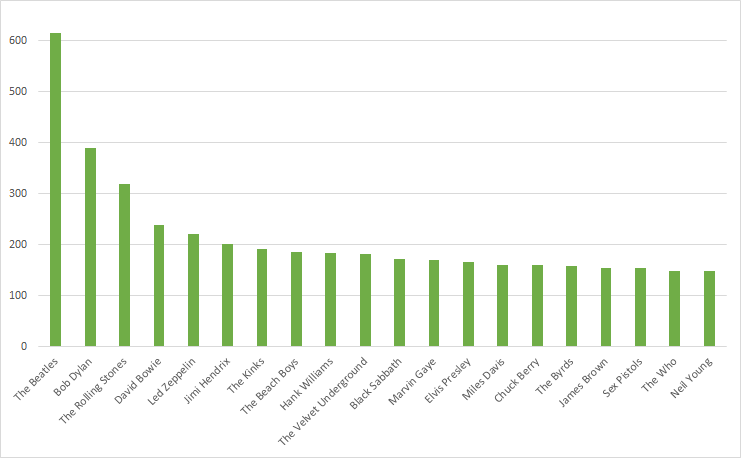
\includegraphics[width=.8\textwidth]{Direct Influence Top.png}
\caption{Number of artists who have direct influence}\label{fig:Direct Influence Top}
\end{figure}

% \section{Appendix B: Program Codes}
% Here are the program codes we used in our research.

% 代码环境示例三则
% 如您的论文不需要展示代码,请删除
% 更多用法,请参考 listings 宏包文档

% Python 代码示例
% \begin{lstlisting}[language=Python, name={test.py}]
% # Python code example
% for i in range(10):
%     print('Hello, world!')
% \end{lstlisting}

% MATLAB 代码示例
% \begin{lstlisting}[language=MATLAB, name={test.m}]
% % MATLAB code example
% for i = 1:10
%     disp("hello, world!");
% end
% \end{lstlisting}

% C++ 代码示例
% \begin{lstlisting}[language=C++, name={test.cpp}]
% // C++ code example
% #include <iostream>
% using namespace std;

% int main() {
%     for (int i = 0; i < 10; i++)
%         cout << "hello, world" << endl;
%     return 0;
% }
% \end{lstlisting}

\end{subappendices}  

\end{document}  
